% !TeX root = SketchFace.tex

\subsubsection{Spatial Attention Pooling}
When the input hand-drawn sketch is not well-drawn, it is a trade-off between the realism of the output face image and the alignment between the input sketch and the output face image.
%
In order to alleviate the edge alignment between the input sketch and the output face image, we should relax the sharp sketch lines with one-pixel width.
\cxj{relax thin strokes to an ambiguity band with various width or uncertainty.}
One of the straightforward ways is to smooth the lines of sketches using image smoothing algorithm. 
Another is to dilate the sketch lines so that the widths of lines are of multiple pixels~\cite{DeepSurgery}.
\cxj{if it is not officially published, it is not necessary to cite it. but if our method performs better, then cite it and show comparison.}
However, the capacity of either the two hand-crafted ways above is limited, \td{because the uniform smoothness and the dilate radius for all positions of the whole sketch violate the unevenness of hand-drawn sketches on depicting different facial parts. }
%
We argue that the balance between the realism of the output face image and the alignment between the input sketch and the output face image differs from one position to another across the face image. Therefore, the smoothness or the dilation radius should be spatial-specific. 

Based on the discussion above, we propose a new module, called spatial attention pooling (SAP), to dilate the input sketch in a spacial-specific way. 
\cxj{I would not use 'dilate' since this simple word does not reveal the underlying discovery.}
%Let $\mathbf{r}=\{r_i | i=1,2,...,N_r\}$ be a set of dilation radius. 
Given an input sketch $S\in \real^{H\times W}$, we first pass it through $N_r$ pooling branches with different kernel sizes of $r_i, i=1,\ldots, N_r$ to get $\{P_{i}| i=1,\ldots,N_r\}$. 
Then we compute the spatial attention map $W\in \real^{N_r\times H\times W} $with $W = Softmax(f(s))$, where $f()$ is implemented with two convolutional layers. \cxj{$f(S)$ to extract low-level features from the input sketch?}
\cxj{It is not clear what is the motivation of computing the SA map $W$. It might be better to describe your idea of how to use $W$ with $P$ and then describe how to get $W$. }
%
A softmax layer which is computed over channels is added at the end of the convolutional layers, ensuring that for each position, the sum of weights of all channels equals to $1$. The output of SAP is computed as:
	
\begin{equation}
	SAP(s)=\sum_{i=1}^{N_r} W_i * P_{r_i}(s),
\end{equation}
%
where $W_i$ is the $i$th channel of $W$, \td{and $*$ is element-wise multiplication}.
\td{We show this idea in Fig.~\ref{fig:sap}.}

\begin{figure}
	\centering
	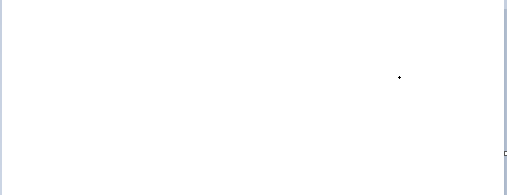
\includegraphics[width=\columnwidth]{figs/box.png}
	\caption{Spatial attention pooling to balance edge alignment and stroke ambiguity at different facial regions. }
	\label{fig:sap}
\end{figure}


